% Multiple Integrals 400: the triangle below y = x (from Lab 11).
\documentclass[border=4pt]{standalone}
\usepackage{tikz}
\begin{document}
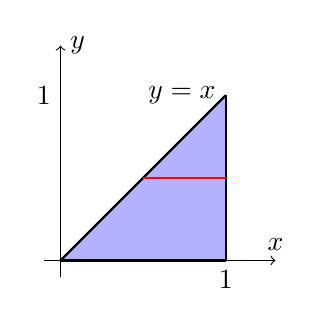
\begin{tikzpicture}[scale=2.1]
  \draw[->] (-0.1,0) -- (1.3,0) node[above] {$x$};
  \draw[->] (0,-0.1) -- (0,1.3) node[right] {$y$};
  \fill[blue!30] (0,0) -- (1,0) -- (1,1) -- cycle;
  \draw[thick] (0,0) -- (1,1) node[left] {$y=x$};
  \draw[thick] (0,0) -- (1,0);
  \draw[thick] (1,1) -- (1,0);
  \draw[thick, red] (.5,.5) -- (1,.5);
  \draw (1,0) -- (1,1);
  \node[below] at (1,0) {$1$};
  \node[left]  at (0,1) {$1$};
\end{tikzpicture}
\end{document}
